\chapter{绪论}
\section{推荐系统的研究背景}
近些年,随着信息科技的广泛应用和迅猛发展,互联网正在渗透我们日常生活中的各个方面,
人们逐渐从信息匮乏的时代走入了信息过载(Information Overload)的时代。
为了解决信息过载的问题,诸多富有创造力的解决方案被提出,
其中最具代表性的是分类目录,搜索引擎和推荐系统(Recommender System)。
采用分类目录方案的代表包括国外的雅虎和国内的Hao123,它们的核心功能是将流行的网站分门别类,
为用户提供免费的网站导航,将用户引导至感兴趣的网站上。
但随着互联网规模的不断扩大,分类目录网站覆盖的少量热门网站也越来越难以满足用户的需求,
搜索引擎技术应运而生。著名的搜索引擎网站包括国外的谷歌和国内的百度,
通过这些网站,用户只需要输入几个关键词就可以获取高度相关的信息。
和搜索引擎一样,推荐系统也是一种帮助人们快速寻找感兴趣信息的解决方案,
不同的是,推荐系统不需要用户提供明确的信息需求,而是通过用户的历史行为进行兴趣建模,
从而提供满足用户兴趣的信息。可以说搜索引擎和推荐系统相辅相成,
一个满足了用户有明确信息需求时的信息检索,
另一个满足了用户没有明确信息需求时的信息推荐。

\begin{figure}[htbp]
\centering
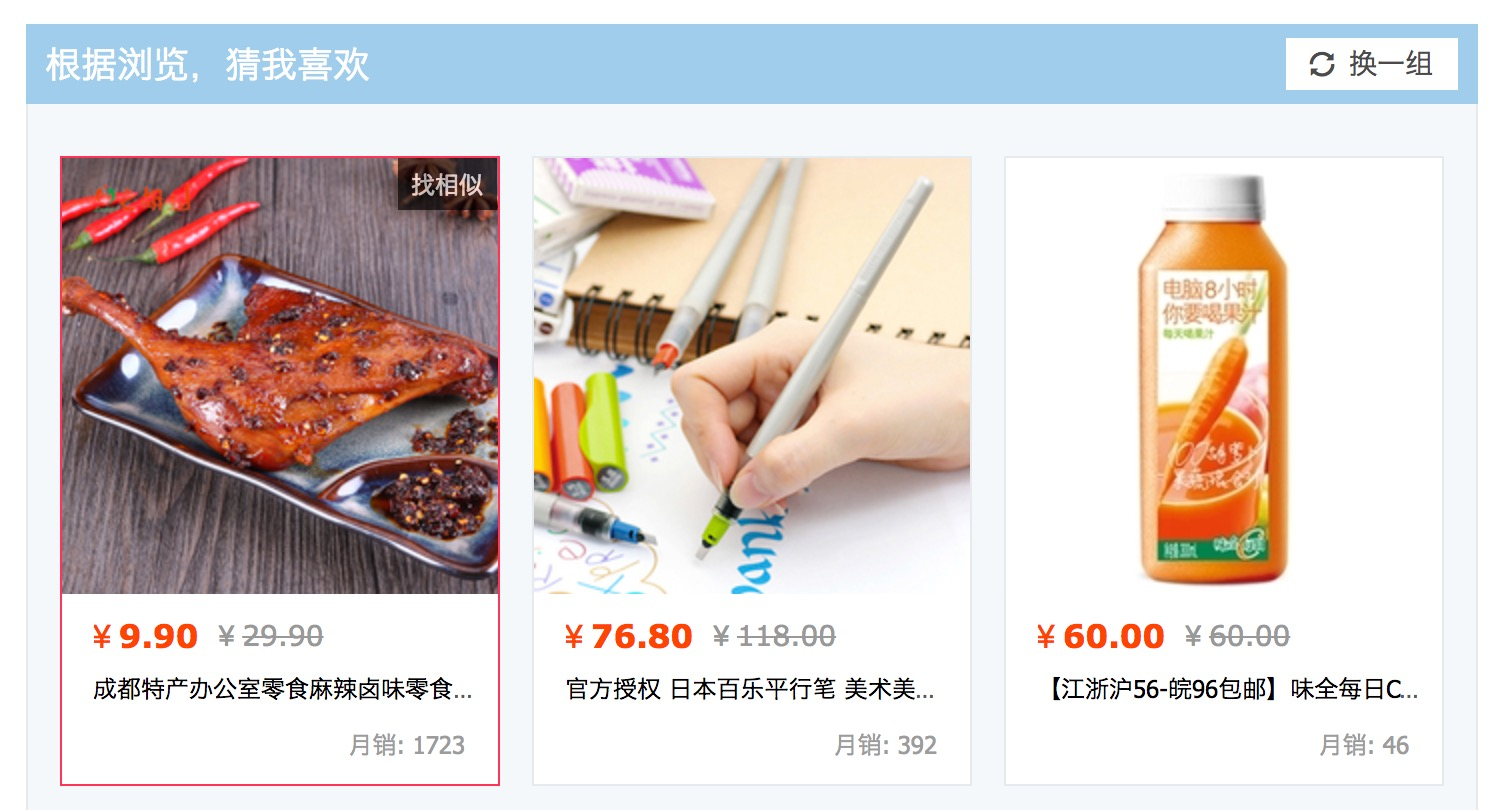
\includegraphics[scale=0.26]{images/taobao.jpeg}
\caption{淘宝网上的商品推荐样例}
\label{fig:taobao}
\end{figure}

千禧年伊始,互联网逐渐从以编辑为主体的Web1.0时代进入以用户为主体的Web2.0时代,
大量用户生成数据充斥着网络,信息爆炸式地增长,标志着大数据时代的到来。
电商平台里的商品、媒体网站里的新闻、小说网站里的作品、招聘网站里的职位等,
当数量超过用户可以遍历的上限时,用户开始无法快速获取满足他们需求的信息。
推荐系统可以对海量信息进行筛选过滤,将用户最关注最感兴趣的信息展现在用户面前,
能大大增加这些内容的转化率,对各类应用系统都有非常巨大的价值,
逐渐成为互联网平台不可或缺的一环。
图\ref{fig:taobao}给出了著名电子商务网站淘宝网上的商品推荐样例。

一般认为,推荐系统成为一个相对独立的研究方向始于1994年美国
明尼苏达大学GroupLens研究组推出GroupLens系统\parencite{resnick1994grouplens},
该系统主要有两大重要贡献,一是为推荐问题创建了一个形式化的数学模型,
二是首次提出了基于协同过滤方法完成推荐任务的思想。
该系统提出的模型属于一种基于用户的协同过滤算法,
之后的几十年,其他一些协同过滤的算法也相继被提出,
其中最具代表性的是基于物品的协同过滤算法和基于矩阵分解的协同过滤算法。
2006年著名的互联网公司Netflix举办的百万美金大奖赛可以看做是推荐系统的一次热潮。
全球四万多个团队参赛,经过近三年的较量,获奖队伍终于达到了比赛的设定条件。
其使用的方法的核心模块就是矩阵分解,
这使得基于矩阵分解的协同过滤在近十年中得到了学术界和工业界的广泛关注和重视。
同时,其他推荐算法也在不断发展,比如基于内容的推荐,
基于知识库的推荐,以及借助情感分析和主题模型的基于文本的推荐等等。
另外,这些方法之间的互补与融合也成为了重要的研究方向。

\section{深度学习的研究背景}
深度学习(Deep Learning)起源于人工神经网络的研究,是今年来兴起的机器学习范式,
拥有多个隐层的多层感知器(Multi-Layer Perceptron)就是一种深度学习模型。
深度学习利用其多层神经网络结构,通过底层基础特征学习抽象的高层表示特征,
直接尝试解决抽象认知的难题,在语音识别、图像识别和自然语言处理等研究领域取得了突破性的进展。

反向传播算法作为人工神经网络最初的训练算法,由于训练过程中存在梯度消失或梯度爆炸的问题,
以及容易陷入局部最优值的不足,被人们所遗弃。
2006年,Hinton等人\parencite{hinton2006fast}提出深度置信网络(Deep Belief Nets),
通过逐层预训练的方法,为神经网络提供一个较优的初始值,然后进行微调完成训练过程,
从而解决了反向传播算法带来的优化难题。

Lecun等人\parencite{lecun1989backpropagation}提出卷积神经网络
(Convolutional Neural Network),利用空间相对关系减少参数数目以提高训练性能,
并将其成功应用于图像处理领域,在手写字体识别、图像分割和物体检测等研究领域取得了突破性的进展。
围棋项目上,AlphaGo结合卷积神经网络和蒙特卡洛树搜索,成功击败人类著名棋手李世石,
引爆了深度学习的热潮,将人工智能带上了一个新的台阶。深度学习不仅学术意义巨大,
而且实用性很强,工业界也开始了大规模的投入,大量新型产品从中获益。
例如著名电动汽车公司特斯拉推出自动驾驶汽车,在一定程度上能减轻驾驶人员负担,
不仅可帮助减少车祸,还能大幅降低交通拥堵情况。

自然语言处理与深度学习的初次结合来源于2013年
Mikolov等人\parencite{mikolov2013efficient}提出的Word2Vec模型,
从提出至今,Word2Vec已经成为了深度学习在自然语言处理中的基础部件,
不胜枚举的深度学习模型在表示单词、短语、句子、段落等文本要素时都需要用Word2Vec来做单词级别的向量化。
此后深度学习在自然语言处理领域大显神威,在情感分析、问答系统、机器翻译等问题上,
以惊人的效果提升,颠覆了使用多年的老方法。
更重要的是,它引起了对主流方法的反思,提供了一个全新的思考视角。

\section{本文主要工作及成果}
受到深度学习在自然语言处理领域的成功应用的启发,本文尝试将深度学习和推荐系统进行结合,
利用深度学习能够高效学习高层抽象的特点,对用户和物品进行更加准确地建模。与此同时,
本文考虑到用户的兴趣分布会随时间流逝发生变化的特点,提出长短期兴趣模型,
在学习过程中融入了时间因素,使得用户模型和物品模型更加具有时效性,从而进一步提升推荐系统的推荐性能。

\section{本文篇章结构}
本文一共由五个章节组成。
第一章节是绪论部分,主要介绍了本文的研究背景及意义,阐述了推荐系统的问题定义,包括数据集和评价方法等,
然后介绍了我们的工作和研究成果,最后描述了本文的篇章结构。
第二章节。
第三章节。
第四章节。
最后,第五章节对本文的研究工作进行了总结与归纳,并对未来可能的拓展方向进行了展望。


